\RequirePackage{fixltx2e}
\documentclass{jknotes}
\usepackage{joshkirklin}

\begin{document}

\institution{Cambridge Part III Maths}
\title{Black Holes}
\lecturer{Harvey Reall}
\notetaker{Josh Kirklin}
\date{Lent 2016}

\maketitle
\suggestionsspiel
In this course we take \(G=c=1\) and \(\Lambda=0\).
\tableofcontents

\section{Spherical stars}
\lecture{15/01/16}
Consider a gas of cold fermions. This gas will resist compression due to \emph{degeneracy pressure} resulting from the Pauli principle. For example, in a white dwarf star, gravity is balanced by electron degeneracy pressure. Using Newtonian gravity, we can find an upper limit on the mass of a stable white dwarf, known as the \emph{Chandrasekhar limit}:
\begin{equation}
    M_{\text{WD}} \lesssim 1.4M_{\astrosun}
\end{equation}

In a neutron star, gravity is balanced by neutron degeneracy pressure. Neutron stars are tiny; a neutron star with the mass of the sun has a radius of approximately \SI{10}{\kilo\meter} (for comparison, the sun has a radius of \(R_{\astrosun}\approx\SI{7e5}{\kilo\meter}\). At the surface of a neutron star, the gravitational potential \(|\phi|\approx0.1\). Recall that in order to be able to apply Newtonian gravity, we must have \(|\phi|\ll1\). \(0.1
\not\ll1\), so it is important to consider general relativity when reasoning about neutron stars.

In this section we will establish that \(M \lesssim 3M_{\astrosun}\) for \emph{any} cold star.

\subsection{Spherical symmetry and time independence}

Consider the round metric on \(S^2\):
\begin{equation}
    \dd{\Omega}^2 = \dd{\theta}^2+\sin^2\theta\dd{\phi}^2
\end{equation}
Equipped with this metric, if we exclude reflections, \(S^2\) has \(SO(3)\) as its isometry group. This motivates the following:
\begin{defn}
    A spacetime is \emph{spherically symmetric} if its isometry group has an \(SO(3)\) subgroup whose orbits are 2-spheres.
\end{defn}
\begin{defn}
    The \emph{area-radius function} \(r:\mathcal{M}\rightarrow\RR\) is defined by:
    \begin{equation}
        A(p) = 4\pi r(p)^2,\quad r(p)\ge 0
    \end{equation}
where \(A(p)\) is the area of the \(SO(3)\) orbit through \(p\).
\end{defn}
A consequence of this is that the induced metric on the \(SO(3)\) orbit through \(p\) is \(r(p)^2\dd{\Omega}^2\).

\begin{defn}
    \((\mathcal{M},g)\) is \emph{stationary} if it permits a timelike Killing vector field (KVF).
\end{defn}

\begin{wrapfigure}{L}{0.3\textwidth}
    \centering
    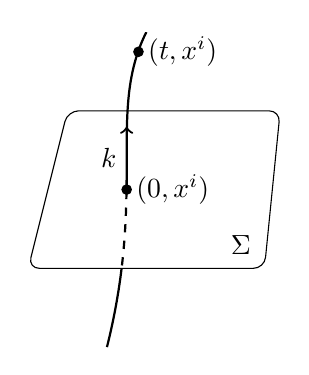
\begin{tikzpicture}
        \draw[rounded corners] (0,0) -- (0.5,2) -- (3.2,2) -- (3,0) -- cycle;
        \def\killingone{\draw[thick] (1,-1) .. controls (1.5,1) and (1,2) .. (1.5,3)}
        \begin{scope}
            \clip (0,0) rectangle (3,-1);
            \killingone;
        \end{scope}
        \begin{scope}[dashed]
            \clip (0,1) rectangle (3,0);
            \killingone;
        \end{scope}
        \begin{scope}
            \clip (0,1) rectangle (3,3);
            \killingone;
        \end{scope}
        \draw[fill] (1.25,1) circle (0.06) node[right] {\((0,x^i)\)};
        \draw[->,thick] (1.25,1) -- (1.25,1.8) node[midway,left] {\(k\)};
        \draw[fill] (1.4,2.75) circle (0.06) node[right] {\((t,x^i)\)};
        \node at (2.7,0.3) {\(\Sigma\)};
    \end{tikzpicture}
\end{wrapfigure}

Suppose we have a stationary spacetime with timelike Killing vector \(k\). Let \(\Sigma\) be a spacelike 3 dimensional hypersurface, and let \(x^i\), \(i=1,2,3\) be coordinates on \(\Sigma\).

We define coordinates for the manifold in the following way: from each point \((x^1,x^2,x^3)\) extend an integral curve of \(k\); the point \((t,x^i)\) is a parameter distance \(t\) along this curve.

In the chart \((t,x^i)\), we can write:
\begin{equation}
    k=\pdv{t}
\end{equation}
Then, using the defining property of Killing vectors, we have that the metric is independent of \(t\). Thus, we can write:
\begin{equation}
    \dd{s}^2 = g_{00}(x^k)\dd{t}^2 + 2g_{0i}(x^k)\dd{t}\dd{x^i} + g_{ij}(x^j)\dd{x^i}\dd{x^j}
\end{equation}
and we have \(g_{00}<0\) since \(k\) is timelike.

Suppose we have a surface \(\Sigma\) given by \(f(x)=0\), where \(f:\mathcal{M}\rightarrow\RR\), \(\dd{f}|_\Sigma\ne0\). Then \(\dd{f}\) is normal to \(\Sigma\). Suppose \(n\) is another 1-form that is normal to \(\Sigma\). Then we can write \(n=g\dd{f}+fn'\), where \(g\) is a function and \(n'\) is some 1-form. We have:
\begin{equation}
    \dd{n} = \dd{g}\wedge\dd{f}+g\underbrace{\dd[2]{f}}_{=0} + \dd{f}\wedge n' + f\dd{n'}
\end{equation}
\begin{equation}
    \implies \dd{n}|_\Sigma = (\dd{g}-n')\wedge\dd{f} \implies n\wedge \dd{n}|_\Sigma = 0
\end{equation}
In fact, the converse is true:
\begin{theorem}[Frobenius]
    If \(n\) is a 1-form such that \(n\wedge \dd{n}=0\), then there exist functions \(f,g\) such that \(n=g\dd{f}\), so that \(n\) is normal to surfaces of constant \(f\).
\end{theorem}
If \(n\) is a 1-form of this type, we say it is \emph{hypersurface-orthogonal}.

\begin{defn}
    \((\mathcal{M},g)\) is \emph{static} if it contains a hypersurface-orthogonal timelike KVF.
\end{defn}

Suppose we are in a static spacetime, and define coordinates \(t,x^i\) as before. \(\Sigma\) is a surface of constant \(t\), so we have \(k \propto dt\), \(k_\mu \propto (1,0,0,0)\). Also note that \(k_\mu = g_{\mu\nu}k^\nu = g_{\mu\nu}(\pdv{t})^\nu = (g_{00},g_{10},g_{20},g_{30})\). Hence we can deduce that \(g_{i0}=0\), and can write the metric as:
\begin{equation}
    \dd{s}^2 = g_{00}(x^k) \dd{t}^2 + g_{ij}(x^k)\dd{x^i}\dd{x^j}
\end{equation}
where as before \(g_{00}<0\). In this metric we have a discrete isometry \((t,x^i) \rightarrow (-t,x^i)\). A static metric must be time-independent \emph{and} invariant under time reversal. A simple case of a stationary but not static metric is that associated with a rotating star. If we reverse time the star spins in the other direction.

\subsection{Static, spherically symmetric spacetimes}
If we have a spacetime that is both stationary and spherically symmetric, then the isometry group must contain:
\begin{equation}
    \underbrace{\RR}_{\substack{\text{time}\\\text{translation}}} \times \underbrace{SO(3)}_{S^2 \text{ orbits}}
\end{equation}
It can be shown that with this condition the spacetime must also be static.

Let \(\Sigma_t \perp k^a\) be a foliation of the spacetime, and use coordinates \((r,\theta,\phi)\) on each surface, where \(\theta,\phi\) are the usual spherical coordinates and \(r\) is the area-radius function as defined earlier. Then we must have:
\begin{equation}
    \dd{s}^2|_{\Sigma_t} = e^{2\Psi(r)}\dd{r}^2 + r^2\dd{\Omega}
\end{equation}
for some function \(\Psi(r)\). Note that we have no \(\dd{r}\dd{\theta}\) or \(\dd{r}\dd{\phi}\) terms because they would violate spherical symmetry. If we define \(t\) as above we can then write the entire metric as:
\begin{equation}
    \dd{s}^2 = -e^{2\Phi(r)}\dd{t}^2 + e^{2\Psi(r)}\dd{r}^2 + r^2\dd{\Omega}
\end{equation}
for some other function \(\Phi(r)\).

Consider noe the matter inside a stationary and spherically symmetric star. We will model the star as a perfect fluid, which means we have the following energy-momentum tensor:
\begin{equation}
    T_{ab} = (\rho+P)u_au_b + \rho g_{ab}
\end{equation}
where \(\rho\) is the energy density, \(P\) is the pressure, and \(u_a\) is the 4-velocity of the fluid. Since the star is stationary, we can assume the fluid is at rest, so \(u^a = e^{-\Phi}\left( \pdv{t} \right)^a\) (since \(u\) is a unit vector pointing in the \(t\) direction). Also, since we have spherical symmetry we can assume that \(\rho\) and \(P\) are functions of \(r\) only.

\end{document}
